% Options for packages loaded elsewhere
\PassOptionsToPackage{unicode}{hyperref}
\PassOptionsToPackage{hyphens}{url}
%
\documentclass[
]{article}
\usepackage{amsmath,amssymb}
\usepackage{iftex}
\ifPDFTeX
  \usepackage[T1]{fontenc}
  \usepackage[utf8]{inputenc}
  \usepackage{textcomp} % provide euro and other symbols
\else % if luatex or xetex
  \usepackage{unicode-math} % this also loads fontspec
  \defaultfontfeatures{Scale=MatchLowercase}
  \defaultfontfeatures[\rmfamily]{Ligatures=TeX,Scale=1}
\fi
\usepackage{lmodern}
\ifPDFTeX\else
  % xetex/luatex font selection
\fi
% Use upquote if available, for straight quotes in verbatim environments
\IfFileExists{upquote.sty}{\usepackage{upquote}}{}
\IfFileExists{microtype.sty}{% use microtype if available
  \usepackage[]{microtype}
  \UseMicrotypeSet[protrusion]{basicmath} % disable protrusion for tt fonts
}{}
\makeatletter
\@ifundefined{KOMAClassName}{% if non-KOMA class
  \IfFileExists{parskip.sty}{%
    \usepackage{parskip}
  }{% else
    \setlength{\parindent}{0pt}
    \setlength{\parskip}{6pt plus 2pt minus 1pt}}
}{% if KOMA class
  \KOMAoptions{parskip=half}}
\makeatother
\usepackage{xcolor}
\usepackage[margin=1in]{geometry}
\usepackage{graphicx}
\makeatletter
\def\maxwidth{\ifdim\Gin@nat@width>\linewidth\linewidth\else\Gin@nat@width\fi}
\def\maxheight{\ifdim\Gin@nat@height>\textheight\textheight\else\Gin@nat@height\fi}
\makeatother
% Scale images if necessary, so that they will not overflow the page
% margins by default, and it is still possible to overwrite the defaults
% using explicit options in \includegraphics[width, height, ...]{}
\setkeys{Gin}{width=\maxwidth,height=\maxheight,keepaspectratio}
% Set default figure placement to htbp
\makeatletter
\def\fps@figure{htbp}
\makeatother
\setlength{\emergencystretch}{3em} % prevent overfull lines
\providecommand{\tightlist}{%
  \setlength{\itemsep}{0pt}\setlength{\parskip}{0pt}}
\setcounter{secnumdepth}{-\maxdimen} % remove section numbering
\usepackage{amsmath,epsfig}
\usepackage{amssymb,amsthm}
\usepackage[all]{xy}
\usepackage{xcolor}
\usepackage{mathtools}
\usepackage{mathrsfs}
% Needed to have supplementary figures labled as 'S1', 'S2', etc.
\newcommand{\beginsupplement}{
  \setcounter{table}{0}  
  \renewcommand{\thetable}{S\arabic{table}} 
  \setcounter{figure}{0} 
  \renewcommand{\thefigure}{S\arabic{figure}}
}
\newtheorem{lemma}{Lemma}
\newtheorem{theorem}{Theorem}

\usepackage{tabularx}
\usepackage{makecell}
\usepackage{multirow}

% uncomment the following lines for line numbers
\usepackage[left]{lineno}
\linenumbers

% allow for landscape pages
\usepackage{lscape}
\newcommand{\blandscape}{\begin{landscape}}
\newcommand{\elandscape}{\end{landscape}}
\usepackage{float}
\ifLuaTeX
  \usepackage{selnolig}  % disable illegal ligatures
\fi
\usepackage{bookmark}
\IfFileExists{xurl.sty}{\usepackage{xurl}}{} % add URL line breaks if available
\urlstyle{same}
\hypersetup{
  pdftitle={Fast-lived Vertebrate Hosts Exhibit Higher Potential for Mosquito-borne Parasite Transmission},
  pdfauthor={Kyle Dahlin, Suzanne O'Regan, JP Schmidt, Barbara Han, John Drake},
  hidelinks,
  pdfcreator={LaTeX via pandoc}}

\title{Fast-lived Vertebrate Hosts Exhibit Higher Potential for
Mosquito-borne Parasite Transmission}
\author{Kyle Dahlin, Suzanne O'Regan, JP Schmidt, Barbara Han, John
Drake}
\date{October 20, 2024}

\begin{document}
\maketitle

\begin{center}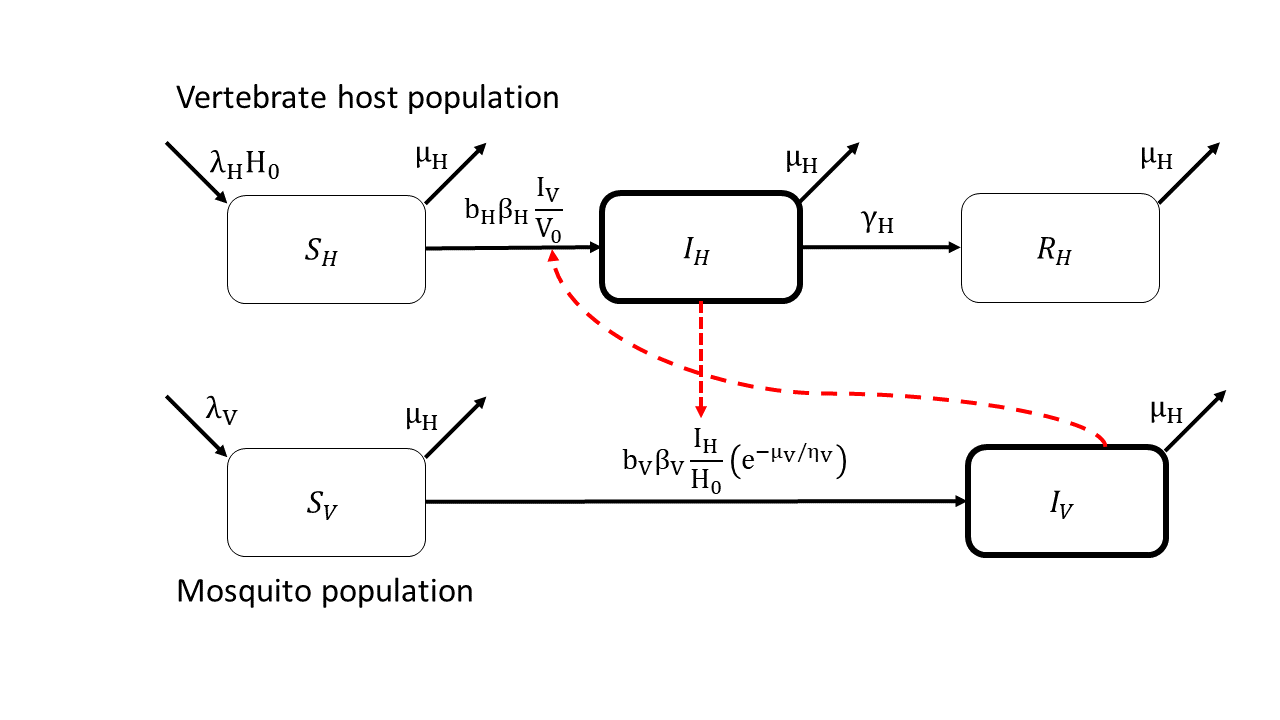
\includegraphics[width=1\linewidth,]{results/flow_diagram} \end{center}

\begin{center}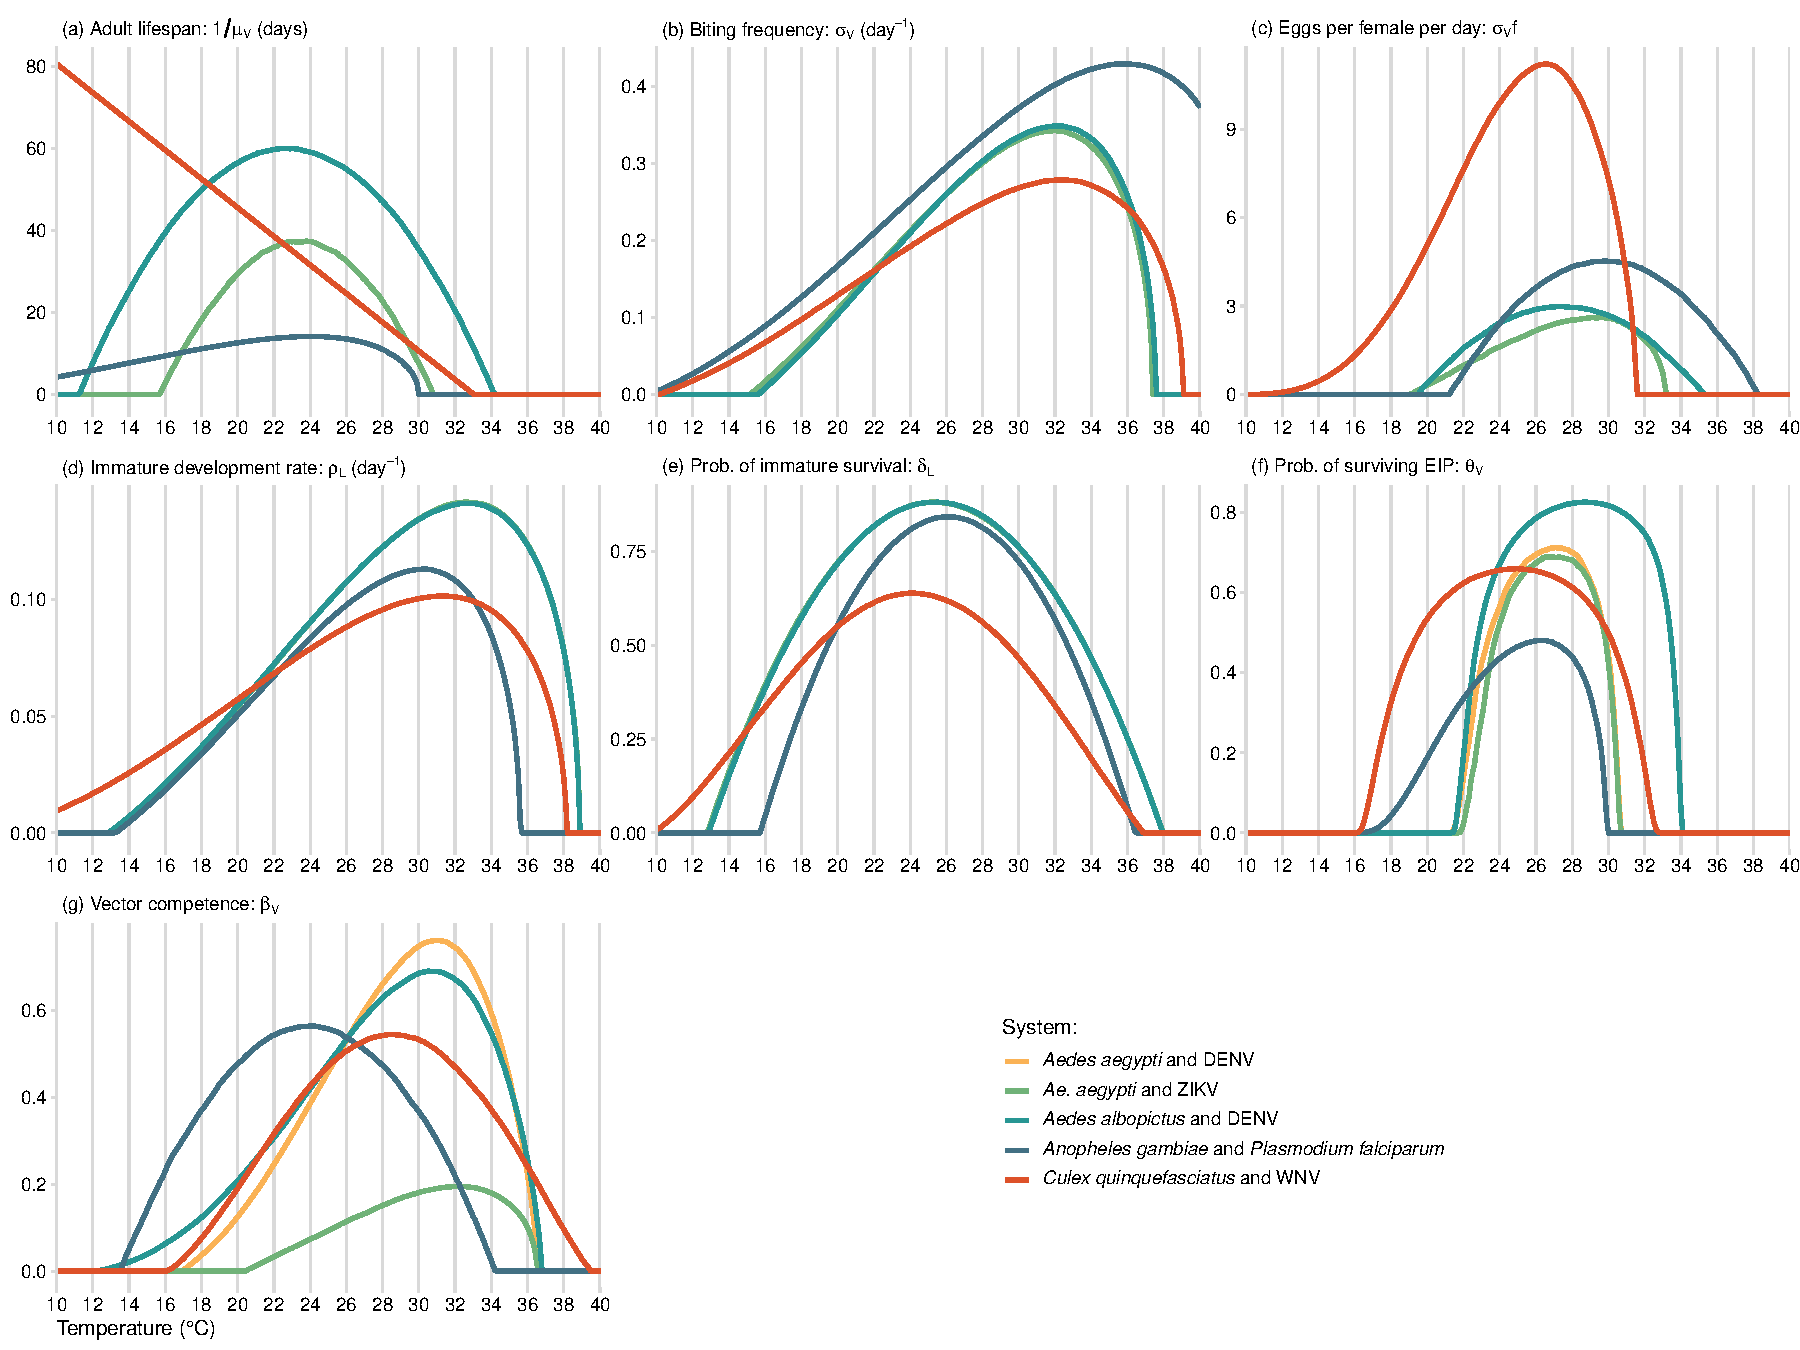
\includegraphics[width=1\linewidth,]{F:/GitHub/GlobalZoonoses-MosquitoSpillover/doc/manuscript-PoLH_files/figure-latex/Fig_S3_Mosquito_TPCs-1} \end{center}

\begin{center}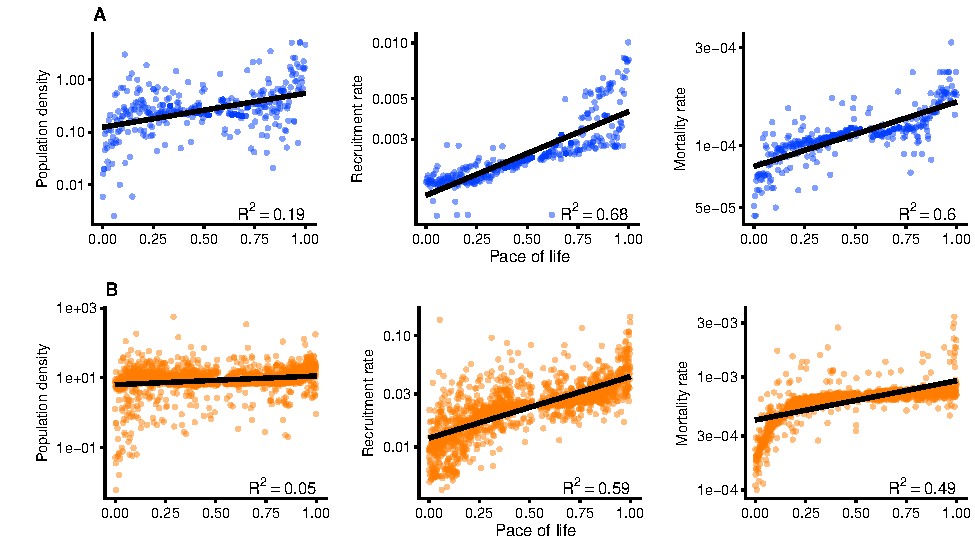
\includegraphics[width=1\linewidth,]{F:/GitHub/GlobalZoonoses-MosquitoSpillover/doc/manuscript-PoLH_files/figure-latex/Fig_2_Trait_Fits-1} \end{center}

\begin{center}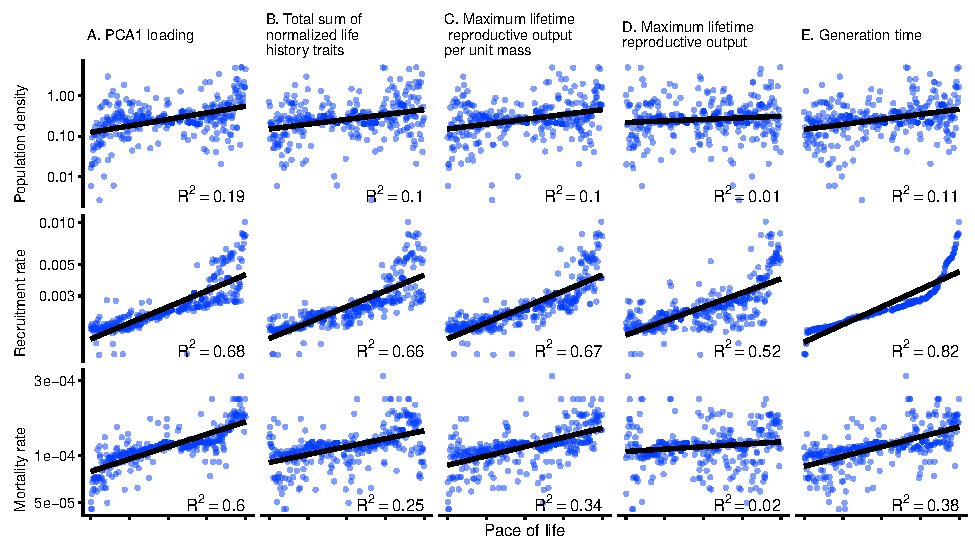
\includegraphics[width=1\linewidth,]{F:/GitHub/GlobalZoonoses-MosquitoSpillover/doc/manuscript-PoLH_files/figure-latex/Fig_S1_Primate_Trait_Fits-1} \end{center}

\begin{center}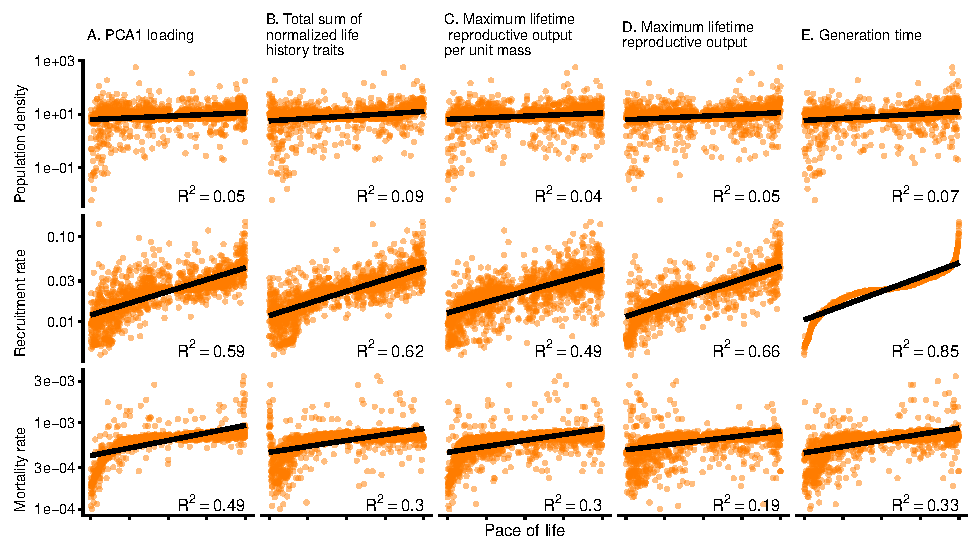
\includegraphics[width=1\linewidth,]{F:/GitHub/GlobalZoonoses-MosquitoSpillover/doc/manuscript-PoLH_files/figure-latex/Fig_S2_Rodent_Trait_Fits-1} \end{center}

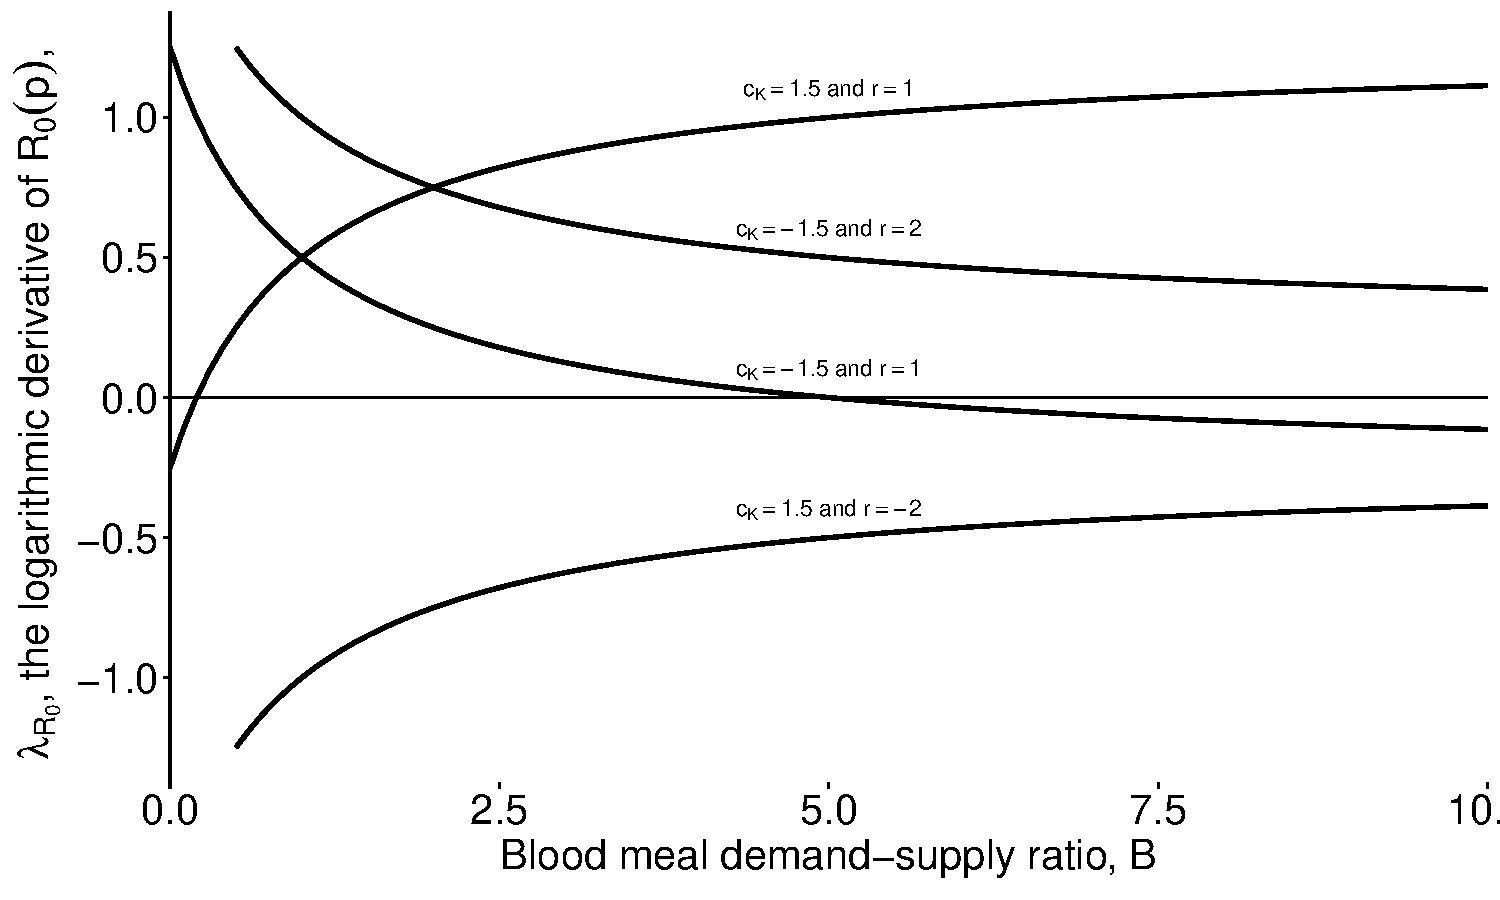
\includegraphics[width=1\linewidth,]{F:/GitHub/GlobalZoonoses-MosquitoSpillover/doc/manuscript-PoLH_files/figure-latex/Fig_S4_lambdaR0_B-1}

\begin{center}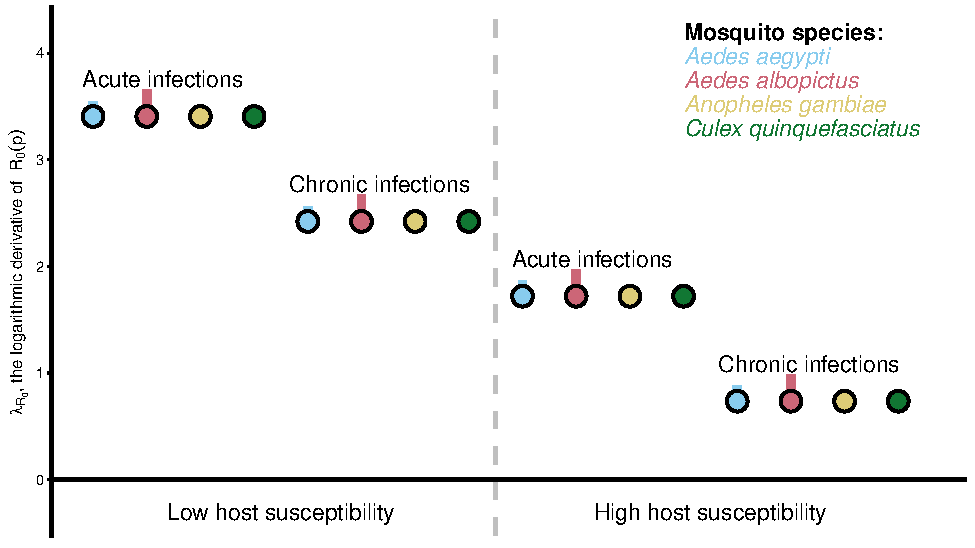
\includegraphics[width=1\linewidth,]{F:/GitHub/GlobalZoonoses-MosquitoSpillover/doc/manuscript-PoLH_files/figure-latex/Fig_3_lambdaR0_Ranges-1} \end{center}

\begin{center}\includegraphics{F:/GitHub/GlobalZoonoses-MosquitoSpillover/doc/manuscript-PoLH_files/figure-latex/Figs_S56_Full_lambdaR0_ranges-1} \end{center}

\end{document}
